\documentclass{article}

\usepackage{fullpage}
\usepackage{amsmath}
\usepackage{amsfonts}
\usepackage{bm}
\usepackage{tabu}
\usepackage{multirow}
\usepackage{graphicx}
\usepackage{grffile}

\newtheorem{theorem}{Theorem}

\newcommand{\Var}{\mathrm{Var}}
\newcommand{\Cov}{\mathrm{Cov}}
\newcommand{\Corr}{\mathrm{Corr}}
\newcommand{\dx}{{\Delta x}}
\newcommand{\dt}{{\Delta t}}
\newcommand{\dV}{{\Delta V}}
\newcommand{\nneigh}{{n_\mathrm{neigh}}}
\newcommand{\avgntilde}{{\langle\tilde{n}\rangle}}
\newcommand{\Nc}{{N_\mathrm{c}}}
\newcommand{\nb}{\bar{n}}
\newcommand{\Nav}{{N_\mathrm{av}}}

\begin{document}

\title{Analysis on the Second-Order Statistics of the Equilibrium Distribution}
\date{}
\author{}
\maketitle

\section{Introduction}

For the one-dimensional diffusion equation subject to stochastic flux under periodic boundary condition,
\begin{equation}
\label{spde}
\frac{\partial}{\partial t}n(x,t)
=\chi\frac{\partial^2}{\partial x^2}n(x,t)
+\frac{\partial}{\partial x}\left[
\sqrt{\frac{2\chi n(x,t)}{A}}\bm{\mathcal{W}}(x,t)
\right],
\end{equation}
the following set of stochastic differential equations is obtained by the finite volume method employing the standard three-point stencil:
\begin{equation}
\label{sode}
\frac{d}{dt}n_j(t)=\chi\frac{n_{j+1}(t)+n_{j-1}(t)-2n_j(t)}{\dx^2}
+\frac{1}{\dx}\left(
\sqrt{\frac{2\chi\tilde{n}_{j+\frac12}(t)}{\dV}}W_{j+\frac12}(t)
-\sqrt{\frac{2\chi\tilde{n}_{j-\frac12}(t)}{\dV}}W_{j-\frac12}(t)
\right).
\end{equation}
In Eq.~\eqref{spde}, $n(x,t)$ and $\bm{\mathcal{W}}(x,t)$ denote the number density and a spatio-temporal Gaussian white noise process satisfying $\langle\bm{\mathcal{W}}(x,t)\bm{\mathcal{W}}(x',t')\rangle =\delta(x-x')\delta(t-t')$, respectively.  
$\chi$ and $A$ are the diffusion coefficient and the cross section area of the system, respectively.
In Eq.~\eqref{sode}, $\dV=A\dx$ is the volume of a cell and $W_\bullet(t)$ are Gaussian white noise processes satisfying $\langle W_\bullet(t)W_\bullet(t')\rangle=\delta(t-t')$.
\\

In Eq.~\eqref{sode}, $\tilde{n}_j(t)$ is the center value of cell $j$, which is to be solved, whereas $\tilde{n}_{j+\frac12}(t)$ is the face value between cells $j$ and $j+1$, which is to be approximated by $n_j(t)$ and $n_{j+1}(t)$.
Hence, a certain rule to determine the face value $\tilde{n}(n_1,n_2)$ from two center values $n_1$ and $n_2$ is additionally required.
A natural way would be using Pythagorean means, i.e., the arithmetic mean (AM), the geometric mean (GM), and the harmonic mean (HM):
\begin{align}
&\tilde{n}^\mathrm{AM}(n_1,n_2)=\frac12(n_1+n_2),\\
&\tilde{n}^\mathrm{GM}(n_1,n_2)=\sqrt{n_1 n_2},\\
&\tilde{n}^\mathrm{HM}(n_1,n_2)=\frac{2}{n_1^{-1}+n_2^{-1}}.
\end{align} 
Then, a natural follow-up question would be which one produces physically the most correct answer.
\\

In this report, we attempt to answer this question by presenting a \textit{complete} analysis on the second-order statistics of the equilibrium state generated by Eq.~\eqref{sode}.
The second-order statistics is described by the variance of the cell number density $\Var[n_j]$ and the covariance between cells $\Cov[n_{j_1},n_{j_2}]$, or equivalently by the structure factor $S(k)$.
The latter is the discrete Fourier series of $\langle n_1 n_j\rangle$ normalized by the volume of the system, where the brackets denote the average over the equilibrium distribution.
We derive exact expressions for these quantities and compare them with physically correct answers to determine the best average type for the discretization of the stochastic flux.
In the rest of this section, we present the physically correct answers and then discuss subtle issues in Eq.~\eqref{sode}.

\subsection*{Physically Correct Answers}

In a physical system having equilibrium number density $\nb$ and a total of $\Nc$ cells of volume $\dV$, there are $\Nc\nb\dV$ particles.
Since there is no preference among the cells under periodic boundary condition, the distribution of $(N_1,N_2,\dots,N_\Nc)$, where $N_i$ is the number of particles in cell $i$, obeys the multinomial distribution with equal probability $1/\Nc$.
Hence, the aforementioned quantities are obtained as
\begin{align}
\label{theovar}
&\Var[n_j]=\frac{\Nc-1}{\Nc}\frac{\nb}{\dV},\\
\label{theocov}
&\Cov[n_{j_1},n_{j_2}]=-\frac{1}{\Nc}\frac{\nb}{\dV}\quad(j_1\ne j_2),\\
\label{theoSk}
&S(k)=
\begin{cases}
V\nb^2 & (k=0),\\
\nb & \left(k={\displaystyle\frac{2\pi m}{\Nc\dx}},\;m=1,\dots,N-1\right).
\end{cases}
\end{align}
If the system is infinite, there is no restriction such as the conservation of total number of particles in the system, and the number of particles in a cell becomes independent from the other cells and it obeys the Poisson distribution with mean $\nb\dV$.

\subsection*{Subtle Issues in Eq.~\eqref{sode}}

One obvious distinction between Eq.~\eqref{sode} and the actual physical system is that $n_j(t)$ in Eq.~\eqref{sode} can be any real number whereas the number density in the physical system should be a nonnegative integer divided by $\dV$. 
In other words, the equilibrium distribution generated by Eq.~\eqref{sode} is continuous, whereas that of the physical system is discrete.
Note that, however, as the average number of particles in a cell, $\Nav=\nb\dV$, becomes larger, the discrete distribution based on the Poisson (or multinomial) statistics can be better approimated by a continuous distribution.
\\

Another unphysical feature of Eq.~\eqref{sode} is that $n_j(t)$ can be negative  depending the realizeation of $W_\bullet(t)$.
In this case, $\tilde{n}$ and/or $\sqrt{2\chi \tilde{n}(x,t)}$ may not be well-defined, which leads to the breakdown of a numerical scheme.
Hence, some \textit{ad hoc} remedies should be provided to the averaging rule $\tilde{n}(n_1,n_2)$.
For example, the stochastic flux is zeroed (i.e., $\tilde{n}(n_1,n_2)=0$) when $n_1$ or $n_2$ becomes negative.\footnote{This can prevent the breakdown of a numerical scheme, but negative densities still may occur.}
Note that this issue becomes more serious as $\Nav$ becomes smaller.
\\

Mathematical analysis of Eq.~\eqref{sode} does not seem very straightforward.
The main reason is that the equation contains multiplicative noise such as $\sqrt{2\chi\tilde{n}(n_j(t),n_{j+1}(t))}W_{j+\frac12}$.\footnote{For the case $\Nav\gg 1$, where the fluctuation in the cell number density becomes small, Eq.~\eqref{sode} can be analyzed under the assumption $\tilde{n}(n_1,n_2)\approx \nb$. However, this analysis cannot answer which averaging method for $\tilde{n}$ works better.}
Futhermore, considering that $\tilde{n}(n_1,n_2)$ becomes even more complicated due to an ad hoc remedy for negative densities, mathematical analysis or theoretical investigation seems intractable. 
In this report, we circumvent this difficulty by deriving expressions for the second-order statistics in terms of the average face value
\begin{equation}
\avgntilde=\langle\tilde{n}(n_j,n_{j\pm1})\rangle.
\end{equation}
In other words, all complicated features of $\tilde{n}$ stay inside $\avgntilde$ and the resulting expressions are exact.

\section{Main Theoretical Results}

The main theoretical results of this report are exact expressions for $\Var[n_j]$, $\Cov[n_{j_1},n_{j_2}]$, and $S(k)$, which are given in Theorem~\ref{mainres}.
The derivation is given in Section~\ref{sec_deriv}.

\begin{theorem}
\label{mainres}
If a numerical scheme satisfies the following conditions:
\begin{enumerate}
\item It converges to Eq.~\eqref{sode} in the limit $\dt\rightarrow0$;
\item There are $\Nc$ cells ($n_1,n_2,\dots,n_\Nc$) and periodic boundary condition is used (i.e., $n_{\Nc+1}(t)=n_1(t)$);
\item It is ergodic,
\end{enumerate}
then the second-order statistics for the equilibrium distribution of ($n_1,n_2,\dots,n_\Nc$) generated by the scheme in the limit $\dt\rightarrow0$ is given as follows:
\begin{align}
\label{resvar}
&\Var[n_j]=\frac{\Nc-1}{\Nc}\frac{\avgntilde}{\dV},\\
\label{rescov}
&\Cov[n_{j_1},n_{j_2}]=-\frac{1}{\Nc}\frac{\avgntilde}{\dV}\quad(j_1\ne j_2),\\
\label{resSk}
&S(k)=
\begin{cases}
V\nb^2 & (k=0),\\
\avgntilde & \left(k={\displaystyle\frac{2\pi m}{\Nc\dx}},\;m=1,\dots,N-1\right),
\end{cases}
\end{align} 
where $\nb$ is the equilibrium number density and $\avgntilde$ is the average face value.
\end{theorem}

It is noted that if $\avgntilde$ were replaced by $\nb$, Eqs.~\eqref{resvar}, \eqref{rescov}, and \eqref{resSk} would become identical to the theoretical predictions based on the multinomial distribution.
Hence, by comparing the values of $\avgntilde$ obtained from different averaging methods with the physically correct value $\nb$, the best averaging method may be determined.

\section{\label{sec_deriv}Derivation}

The expressions shown in Theorem~\ref{mainres} are derived in the following three steps.
In the first step, by introducing the correlation coefficient $\zeta$ between two \textit{contiguous} cells, that is,
\begin{equation}
\zeta=\Corr[n_1,n_2],
\end{equation}
we obtain 
\begin{align}
\label{resvar1}
&\Var[n_j]=\frac{1}{1-\zeta}\frac{\avgntilde}{\dV},\\
\label{rescov1}
&\Cov[n_{j_1},n_{j_2}]=\frac{\zeta}{1-\zeta}\frac{\avgntilde}{\dV}\quad(j_1\ne j_2).
\end{align}
Note that the results are expressed in terms of only $\zeta$ and $\avgntilde$ and the covariances between \textit{any} two different cells are identical.
In the second step, from the conservation of the total sum of cell number densities, we show that
\begin{equation}
\label{reszeta}
\zeta=-\frac{1}{\Nc-1}.
\end{equation}
Then, by substituting Eq.~\eqref{reszeta} into Eqs.~\eqref{resvar1} and \eqref{rescov1}, we express the variance and covariances in terms of only $\avgntilde$ as shown in Eqs.~\eqref{resvar} and \eqref{rescov}.
In the last step, we obtain the expression of $S(k)$ in Eq.~\eqref{resSk} from Eqs.~\eqref{resvar} and \eqref{rescov}.

In the derivation, we frequently use the following properties of the equilibrium distribution under periodic boundary condition:
mean values such as $\langle n_j\rangle$ and $\langle \tilde{n}(n_j,n_{j+1})\rangle$ are identical for all cells;
and correlation quantities such as $\Cov[n_{j_1},n_{j_2}]$ and $\Corr[n_{j_1},n_{j_2}]$ are only dependent on the distance between two cells, i.e., $|j_1-j_2|$ (rather than separately dependent on $j_1$ and $j_2$).

\subsection{Variance and Covariances}

Since the results in Theorem~\ref{mainres} are for the limit $\dt\rightarrow 0$, it suffices to show them for the forward Euler scheme, which is written as follows:
\begin{equation}
\label{feuler}
n_j^\mathrm{new} =n_j+\frac{\chi\dt}{\dx^2}(n_{j+1}+n_{j-1}-2n_j)
+\frac{\sqrt{\dt}}{\dx\sqrt{\dV}}\left(
\sqrt{2\chi\tilde{n}_{j+\frac12}}W_{j+\frac12}
-\sqrt{2\chi\tilde{n}_{j-\frac12}}W_{j-\frac12}
\right).
\end{equation}
Here, $n_j$, $n_j^\mathrm{new}$, and $\tilde{n}_{j+\frac12}$ correspond to $n_j(t)$, $n_j(t+\dt)$, and $\tilde{n}(n_j,n_{j+\frac12})$, respectively, and 
$W_{j+\frac12}$ is an independent standard normal random number.

The property that we are going to use is the time invariance of the equilibrium distribution:
if the distribution of $(n_1,n_2,\dots,n_\Nc)$ is in equilibrium, that of $(n_1^\mathrm{new},n_2^\mathrm{new},\dots,n_\Nc^\mathrm{new})$ is also in equilibrium.
Hence, we have
\begin{equation}
\label{prop}
\langle n_{j_1} n_{j_2} \rangle
=\langle n_{j_1}^\mathrm{new} n_{j_2}^\mathrm{new} \rangle.
\end{equation}
From Eq.~\eqref{feuler}, we obtain
\begin{equation}
\label{njnj}
\begin{split}
\langle n_{j_1}^\mathrm{new} n_{j_2}^\mathrm{new} \rangle
=&\langle n_{j_1} n_{j_2} \rangle
+\frac{\chi\dt}{\dx^2}\langle n_{j_1}(n_{j_2+1}+n_{j_2-1}-2n_{j_2})\rangle
+\frac{\chi\dt}{\dx^2}\langle n_{j_2}(n_{j_1+1}+n_{j_1-1}-2n_{j_1})\rangle\\
&+\frac{2\chi\dt}{\dx^2\dV}\left[
\left(\langle\tilde{n}_{j_1+\frac12}\rangle+\langle\tilde{n}_{j_1-\frac12}\rangle\right)\delta_{j_1,j_2}
-\langle\tilde{n}_{j_1-\frac12}\rangle\delta_{j_1,j_2+1}
-\langle\tilde{n}_{j_1+\frac12}\rangle\delta_{j_1,j_2-1}
\right]
+\mathrm{O}(\dt^2).
\end{split}
\end{equation}
From Eq.~\eqref{prop}, we equate terms of order $\dt$ in Eq.~\eqref{njnj}, which can be expressed by $M_{\Delta j}=\langle n_j n_{j+\Delta j}\rangle$ and $\avgntilde=\langle\tilde{n}_{j+\frac12}\rangle$.
For $j_1=j_2$, $j_1=j_2\pm 1$, and $\left|j_1-j_2\right|=\Delta j\ge2$, respectively, we obtain
\begin{align}
\label{M1}
&M_0 - M_1 = \frac{\avgntilde}{\dV},\\
\label{M2}
&M_0+M_2-2M_1=\frac{\avgntilde}{\dV},\\
\label{M3}
&M_{\Delta j-1}+M_{\Delta j+1}-2M_{\Delta j}=0.
\end{align}
From Eqs.~\eqref{M1}, \eqref{M2}, and \eqref{M3}, we have $M_{\Delta j+1} = M_{\Delta j}$ for $\left|\Delta j\right|\ge1$.
Then, since $M_0=\Var[n_j]-\nb^2$, $M_1=\Cov[n_j,n_{j+1}]-\nb^2$, and $\zeta=\Cov[n_j,n_{j+1}]/\Var[n_j]$, we obtain Eqs.~\eqref{resvar1} and \eqref{rescov1} from Eq.~\eqref{M1}.

\subsection{Correlation Coefficient}

From Eq.~\eqref{sode}, the total sum of cell number densities is conserved:
\begin{equation}
\sum_{j=1}^{\Nc}n_j(t)=\Nc\nb.
\end{equation}
By multiplying $n_1(t)$ and taking the equilibrium average, we obtain
\begin{equation}
\Var[n_1]+\sum_{j=2}^\Nc\Cov[n_1,n_j]=0.
\end{equation}
By substituting Eqs.~\eqref{resvar1} and \eqref{rescov1}, we obtain Eq.~\eqref{reszeta}.

\subsection{Structure Factor}

For $k_m=\frac{2\pi m}{\Nc\dx}$ ($m=0,\dots,\Nc-1$), discrete Fourier coefficient $\hat{n}_{k_m}$ and static structure factor $S(k)$ are defined as follows: 
\begin{align}
\label{defnkhat}
&\hat{n}_{k_m} = \frac{1}{\Nc}\sum_{j=1}^\Nc e^{-i\frac{2\pi m j}{\Nc}}n_j,\\
\label{defSkm}
&S(k_m)=V\langle \hat{n}_{k_m} \hat{n}_{k_m}^*\rangle.
\end{align}
To calculate $S(k)$ from the variance and covariance results, we use the following relation between $S(k_m)$ and $\langle n_1 n_j\rangle$, which can be derived from Eqs.~\eqref{defnkhat} and \eqref{defSkm}:
\begin{equation}
\label{relSkmnjnj}
S(k_m)=\frac{V}{\Nc}\sum_{j=0}^{\Nc-1}e^{-i\frac{2\pi m j}{\Nc}}\langle n_1 n_{1+j}\rangle.
\end{equation}
By substituting the following equation, which is obtained from Eqs.~\eqref{resvar} and \eqref{rescov}, into Eq.~\eqref{relSkmnjnj},
\begin{equation}
\langle n_1 n_j \rangle = \nb^2-\frac{\avgntilde}{V}+\frac{\avgntilde}{\dV}\delta_{j,1},
\end{equation}
and using
\begin{equation}
\frac{1}{\Nc}\sum_{j=0}^{\Nc-1}e^{-i \frac{2\pi m j}{\Nc}}=\delta_{m,0},
\end{equation}
we obtain
\begin{equation}
S(k_m)=\left(V\nb^2-\avgntilde\right)\delta_{m,0}+\avgntilde,
\end{equation}
which is equivalent to Eq.~\eqref{resSk}.

\section{Approximation on the Average Face Value}

In this section, we calculate the face average values over the physically correct equilibrium distribution based on the multinomial distribution.
Under the assumption that the equilibrium distribution generated by a numerical scheme is similar to this distribuion, the resulting face average values may be similar to those obtained from the numerical scheme. 

By denoting the numbers of particles in cells 1 and 2 as $N_1$ and $N_2$, respectively, the marginal distribution of $N_1$ and $N_2$ is written as follows:
\begin{equation}
p_\mathrm{mn}(N_1,N_2)=\frac{\mathcal{N}!}{N_1! N_2!(\mathcal{N}-N_1-N_2)!}p_1^{N_1}p_2^{N_2}(1-p_1-p_2)^{\mathcal{N}-N_1-N_2}
\end{equation}
where mn stands for multinomial and the total number of particles in the system and the probabilities of a particle staying in cells 1 and 2 are $\mathcal{N}=\Nc\nb\dV$ and $p_1=p_2=\frac{1}{\Nc}$, respectively.
As Eqs.~\eqref{theovar} and \eqref{theocov} can be calculated from $p_\mathrm{mn}(N_1,N_2)$, the face average value can be calculated as follows:
\begin{equation}
\label{avgntilde_mn}
\langle\tilde{n}\rangle_\mathrm{mn}=
\sum_{N_1=0}^{\mathcal{N}}\sum_{N_2=0}^{\mathcal{N}-N_1}p(N_1,N_2)\;
\tilde{n}\!\left(\frac{N_1}{\dV},\frac{N_2}{\dV}\right).
\end{equation}
For the arithmetic-mean averaging\footnote{In this case, $\avgntilde_\mathrm{mn}$ can be also calculated from $p_\mathrm{mn}(N_1)\sim\mathrm{Binomial}(\mathcal{N},p_1)$}, we obtain the following favorable result:
\begin{equation}
\label{avgntildemnAM}
\langle\tilde{n}^\mathrm{AM}\rangle_\mathrm{mn}=\nb.
\end{equation}
From the inequilities between Pythagorean means, we also have
\begin{equation}
\label{avgntildemnineq}
\langle\tilde{n}^\mathrm{AM}\rangle_\mathrm{mn}
\ge\langle\tilde{n}^\mathrm{GM}\rangle_\mathrm{mn}
\ge\langle\tilde{n}^\mathrm{HM}\rangle_\mathrm{mn}.
\end{equation}
Note that under the assumption that $\avgntilde\approx\avgntilde_\mathrm{mn}$, Eqs.~\eqref{avgntildemnAM} and \eqref{avgntildemnineq} suggest that the arithmetic-mean averaging gives the most physically-correct answer.

\section{Numerical Results}

Parameter values and settings are as follows:
\begin{itemize}
\item $\chi=1$, $\dx=1$, $\Nc=64$, $\dV=5$ and 10 (i.e., $\Nav=5$ and 10)
\item Midpoint predictor-corrector scheme with $\dt=0.01$
\item Remedy for negative densities:
\begin{align}
&\tilde{n}^\mathrm{AM}(n_1,n_2)=\frac12(n_1+n_2) H_\mathrm{s}(\mathrm{min}(n_1,n_2)\dV),\\
&\tilde{n}^\mathrm{GM}(n_1,n_2)=\sqrt{n_1 n_2} H(\mathrm{min}(n_1,n_2)),\\
&\tilde{n}^\mathrm{HM}(n_1,n_2)=\frac{2}{n_1^{-1}+n_2^{-1}} H(\mathrm{min}(n_1,n_2)),
\end{align} 
where $H$ is the Heaviside step function whereas $H_s$ is a smoothed Heaviside function satisfying $H_s(0)\approx 0$ and $H_s(1)\approx 1$.
\item A total of 16 independent runs for standard errors
\end{itemize}
\vspace{3mm}

\noindent By comparing the second and third columns and the fourth and fifth columns in the following tables, it is confirmed that Eq.~\eqref{resvar} and Eq.~\eqref{reszeta} are valid, respectively.
\begin{center}
($N_\mathrm{av}=5$) \\
\vspace{1mm}
{\tabulinesep=1.2mm
\begin{tabu}{|c||c|c||c|c|}
\hline
average type & $\mathrm{Var}[n]$ (SE) & $\displaystyle\frac{\Nc-1}{\Nc}\frac{\avgntilde}{\dV}$ (SE) & $\zeta$ (SE) & $\displaystyle-\frac{1}{\Nc-1}$ \\
\hline
AM & 0.1944 (0.0002) & 0.19530 ($4\times10^{-6}$) & -0.0188 (0.0008) & \multirow{3}{*}{-0.01587} \\
\cline{1-4}
GM & 0.1860 (0.0001) & 0.18677 ($3\times10^{-6}$) & -0.0180 (0.0009) &  \\
\cline{1-4}
HM & 0.1789 (0.0002) & 0.17922 ($9\times10^{-6}$) & -0.0146 (0.0008) &  \\
\hline
\end{tabu}
}
\end{center}

\begin{center}
($N_\mathrm{av}=10$) \\
\vspace{1mm}
{\tabulinesep=1.2mm
\begin{tabu}{|c||c|c||c|c|}
\hline
average type & $\mathrm{Var}[n]$ (SE) & $\displaystyle\frac{\Nc-1}{\Nc}\frac{\avgntilde}{\dV}$ (SE) & $\zeta$ (SE) & $\displaystyle-\frac{1}{\Nc-1}$ \\
\hline
AM & 0.0984 (0.0001) & 0.09844 ($2\times10^{-7}$) & -0.0156 (0.0011) & \multirow{3}{*}{-0.01587} \\
GM & 0.0959 (0.0001) & 0.09595 ($7\times10^{-7}$) & -0.0158 (0.0011) &  \\
HM & 0.0935 (0.0001) & 0.09377 ($2\times10^{-6}$) & -0.0177 (0.0007) &  \\
\cline{1-4}
\cline{1-4}
\hline
\end{tabu}
}
\end{center}

\begin{figure}
\begin{center}
\framebox[1.2\width]{$\Nav=5$}\\
\includegraphics[angle=270,width=0.7\linewidth]{fig3/N5_DIFF_dt0.01_AVG_Sk.eps}
\caption{\label{fig_Sk_Nav5}[$\Nav=5$] The curves of $S(k)$ obtained from different average types are plotted with errorbars corresponding $2\sigma$ of standard error. The corresponding values of $\avgntilde$ are also plotted in the dotted lines.}
\end{center}
\end{figure}

\begin{figure}
\begin{center}
\framebox[1.2\width]{$\Nav=10$}\\
\includegraphics[angle=270,width=0.7\linewidth]{fig3/N10_DIFF_dt0.01_AVG_Sk.eps}
\caption{\label{fig_Sk_Nav10}[$\Nav=10$] The curves of $S(k)$ obtained from different average types are plotted with errorbars corresponding $2\sigma$ of standard error. The corresponding values of $\avgntilde$ are also plotted in the dotted lines.}
\end{center}
\end{figure}

\noindent Figures~\ref{fig_Sk_Nav5} and \ref{fig_Sk_Nav10} show that Eq.~\eqref{resSk} agrees very well with numerical results.  
\\

\noindent Finally, we compare $\avgntilde$ obtained from numerical results with $\avgntilde_\mathrm{mn}$ calculated from Eq.~\eqref{avgntilde_mn}.
It is observed that this approximation clearly reproduces the trend in the values of $\avgntilde$ among different average types.

\begin{center}
{\tabulinesep=1.2mm
\begin{tabu}{|c||c|c||c|c|}
\hline
\multirow{2}{*}{average type} & \multicolumn{2}{c||}{$N_\mathrm{av}=5$} & \multicolumn{2}{c|}{$N_\mathrm{av}=10$} \\
\cline{2-5}
 & $\avgntilde$ (SE) & $\avgntilde_\mathrm{nm}$ & $\avgntilde$ (SE) & $\avgntilde_\mathrm{nm}$ \\
\hline
AM & 0.99198 ($2\times10^{-5}$) & 1       & 0.99990 ($2\times10^{-6}$) & 1       \\
\hline
GM & 0.94863 ($2\times10^{-5}$) & 0.94285 & 0.97468 ($7\times10^{-6}$) & 0.97387 \\
\hline
HM & 0.91032 ($4\times10^{-5}$) & 0.90000 & 0.95260 ($2\times10^{-5}$) & 0.95000 \\
\hline
\end{tabu}
}
\end{center}

\section{Conclusion}

We have derived exact expressions for the second-order statistics of the equilibrium distribution generated by a numerical scheme based on the three-point standard stencil in the limit $\dt\rightarrow0$.
As seen in $S(k)=\avgntilde$ ($k\ne0$), all relevant quantities are expressed in terms of the face value average $\avgntilde$.
Hence, a criterion for the best average type has been suggested: $\avgntilde$ should be close to $\nb$.
In principle, the latter value can be determined by the (marginal) equilibrium distribution $p(n_1,n_2)$ and the averaging method $\tilde{n}(n_1,n_2)$.
Since a different averaging method would generate a different equilibrium distribution, these two cannot be two independent factors for the face value average.
However, numerical results show that $\avgntilde\approx\avgntilde_\mathrm{mn}$, which implies that the approximation of the equilibrium distribution $p(n_1,n_2)$ by the physically correct equilibrium distribution $p_\mathrm{mn}(n_1,n_2)$ based on the multinomial distribution works very well for the second-order statistics.
Then, from Eqs.~\eqref{avgntildemnAM} and \eqref{avgntildemnineq}, we may conclude that the arithmetic-mean average type produces the most similar second-order statistics to the physical system.
However, the fact that the face value average is not so affected by the deviation of the equilibrium distribution from the multinomial statistics also suggests that the equilibrium distribution should be separately checked (e.g., chances of negative number densities). 
\end{document}
